%% Included in decks: slidemage-manual, slidemage-manual-copy
%%

% SlideMage manual, chapter "Working in SlideMage": the AI assistant (the lower part of the
% workspace's right column) (tools/manual/make_screenshots.py, shot chat).
\setSlideVersion{1-0-0+}
\begin{standardframe}{The AI assistant}
	\small
	Below the panels, an assistant reads and changes your slides, unsaved text included. It comes from the \emph{Claude} and \emph{Ollama} plugins (\emph{Settings} $\rightarrow$ \emph{Extensions}); without them SlideMage has none. \emph{Local} or \emph{Cloud} at its top decides where AI tasks run; its arrow opens \emph{AI setup}.
	\par
	\begin{columns}[T,onlytextwidth]
		\begin{column}{0.25\linewidth}
			{\setlength{\fboxsep}{0pt}\fcolorbox{c_primary_gray}{white}{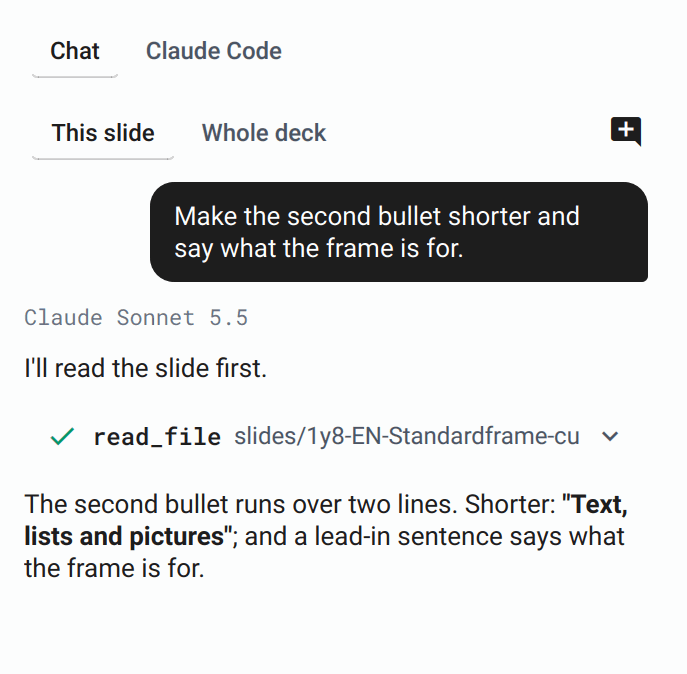
\includegraphics[width=\dimexpr0.8\linewidth-0.8pt\relax]{media/screenshot-slidemage-chat.png}}}
		\end{column}
		\begin{column}{0.37\linewidth}
			\textbf{Chat}
			\shrinklists{3}
			\begin{itemize}
				\item Scope \emph{This slide} (it asks before touching others) or \emph{Whole deck}; a label names the model, local or cloud
				\item Reads, searches and edits files, lints, renders, adds slides, compiles
				\item \emph{Ask before edits} shows a diff to \emph{Apply} or \emph{Reject}; \emph{Edit automatically} applies it, with \emph{Undo}
				\item Header comments, \SMCmd{setSlideVersion} lines, \SMCode{vbox to 0pt} blocks and frozen versions are off limits
			\end{itemize}
		\end{column}
		\begin{column}{0.34\linewidth}
			\textbf{Claude Code}
			\shrinklists{3}
			\begin{itemize}
				\item Your own, logged-in \SMCode{claude}; \emph{AI setup} sets model and effort, \emph{Switch now} applies them, keeping the chat
				\item Sees the focused slide, same limits; asks which version to keep if a file changed on disk
			\end{itemize}
			\textbf{Cloud models}
			\shrinklists{3}
			\begin{itemize}
				\item Need an API key; \emph{Local AI only} (\emph{Settings} $\rightarrow$ \emph{AI}) turns them off; a project asks first what will be sent
			\end{itemize}
		\end{column}
	\end{columns}
\end{standardframe}
